% 字体配置
\ifdefined\freefont
    \usepackage{fontspec}
    \usepackage[fontset=none]{ctex}
    \setmainfont{EB Garamond 12 Regular}[Ligatures={Rare,Historic},Numbers=Lining,BoldFont=[EBGaramond08-Regular]]
    \setmonofont{Maple Mono Normal}

    \newfontfamily\ssfont{Vollkorn Medium Italic}
    \newfontfamily\chenfont{Vollkorn Italic}
    \newfontfamily\pagenfont{Vollkorn Italic}
    \newfontfamily\prenotefonten{EB Garamond 12 Regular}
    \newfontfamily\cpfont{Vollkorn}
    \newfontfamily\scfont{EB Garamond SmallCaps 12 Regular}

    \newfontfamily\mainreg{EB Garamond 12 Regular}[Numbers=Lining,Scale=1.2]
    \newfontfamily\mainsb{Vollkorn}[Numbers=Lining,Scale=1.15]
    \newfontfamily\mainb{Vollkorn Medium}[Scale=1.15,LetterSpace=-1]

    \newfontfamily\titlefonten{Allura}[LetterSpace=1]
    \newfontfamily\tempfont{Source Han Serif CN}

    \setCJKmainfont{Source Han Serif CN}[BoldFont=Source Han Serif CN SemiBold, ItalicFont=FZFangSong-Z02,BoldItalicFont=Source Han Serif CN Bold]
    \setCJKmonofont{FZHei-B01}

    \newCJKfontfamily\elsong{Source Han Serif CN ExtraLight}
    \newCJKfontfamily\lsong{Source Han Serif CN Light}
    \newCJKfontfamily\songti{Source Han Serif CN}
    \newCJKfontfamily\mediumsong{Source Han Serif CN Medium}
    \newCJKfontfamily\sbsong{Source Han Serif CN SemiBold}
    \newCJKfontfamily\bsong{Source Han Serif CN Bold}
    \newCJKfontfamily\hsong{Source Han Serif CN Heavy}

    \newCJKfontfamily\shusong{FZShuSong-Z01}[ItalicFont=FZKai-Z03] % 书宋
    \newCJKfontfamily\fangsong{FZFangSong-Z02} % 仿宋
    \newCJKfontfamily\heiti{FZHei-B01} % 黑体
    \newCJKfontfamily\kaiti{FZKai-Z03} % 楷体


    \newcommand{\titlefont}{\titlefonten\fangsong}
    \newcommand{\signfont}{\writing}

    \newcommand{\tocmain}{\bsong}
    \newcommand{\tocpart}{\sbsong\ssfont}
    \newcommand{\tocchapter}{\sbsong\chenfont}
    \newcommand{\tocchaplabel}{\itshape}
    \newcommand{\tocsection}{\songti}
    \newcommand{\tocsectlabel}{\scfont}
    \newcommand{\tocsubsection}{\tocsection}
    \newcommand{\tocsubsectlabel}{\tocsectlabel}
    \newcommand{\tocpage}{\pagenfont}

    \newcommand{\partfont}{\bsong\mainb}
    \newcommand{\chapterfont}{\bsong\mainb}
    \newcommand{\sectionfont}{\sbsong\mainsb}
    \newcommand{\subsectionfont}{\songti\mainreg}
    \newcommand{\pagenumberfont}{\tocpage}
    \newcommand{\headfont}{\kaiti\cpfont}
    \newcommand{\quotefont}{\itshape}
    \newcommand{\prenotefont}{\prenotefonten\sbsong}
    \newcommand{\writing}{\rmfamily\sbsong}
    \newcommand{\spellfont}{\quotefont}
    \newcommand{\dotfont}{\shusong}
\else
    \usepackage{ctex}
    \newcommand{\prenotefont}{\rmfamily}
    \newcommand{\titlefont}{}
    \newcommand{\signfont}{\ttfamily}
    \newcommand{\cpfont}{\ttfamily}

    \newcommand{\tocmain}{\bfseries}
    \newcommand{\tocpart}{\bfseries}
    \newcommand{\tocchapter}{\itshape}
    \newcommand{\tocchaplabel}{\itshape}
    \newcommand{\tocsection}{\rmfamily}
    \newcommand{\tocsectlabel}{\rmfamily}
    \newcommand{\tocsubsection}{\tocsection}
    \newcommand{\tocsubsectlabel}{\tocsectlabel}
    \newcommand{\tocpage}{\ttfamily}
    \newcommand{\ssfont}{\itshape}

    \newcommand{\partfont}{\bfseries\itshape}
    \newcommand{\chapterfont}{\bfseries}
    \newcommand{\sectionfont}{\bfseries}
    \newcommand{\subsectionfont}{\sffamily}
    \newcommand{\pagenumberfont}{\tocpage}
    \newcommand{\headfont}{\ttfamily}
    \newcommand{\quotefont}{\itshape}
    \newcommand{\writing}{\rmfamily\ttfamily}
    \newcommand{\spellfont}{\quotefont}
    \newcommand{\dotfont}{\rmfamily}
    \newcommand{\tempfont}{\rmfamily}
\fi


% 首段缩进
\usepackage{indentfirst}

% 启用并隐藏超链接
\usepackage{hyperref}
\hypersetup{hidelinks}

% 调整行距为1.618
\usepackage{setspace}
\setstretch{1.618}
% 段距增加弹性
\setlength{\parskip}{0em plus .1\baselineskip}

% 页面配置
\usepackage{geometry}
% 主布局
\newlength{\pw}
\newlength{\ph}
% A5 148*210
\setlength{\pw}{148mm}
\setlength{\ph}{210mm}

\newlength{\bleedlen}
\setlength{\bleedlen}{0mm}

\newlength{\ptop}
\newlength{\pbottom}
\newlength{\pinner}
\newlength{\pouter}
\newlength{\phsep}
\newlength{\pfskip}

\setlength{\ptop}{21mm}
\setlength{\pbottom}{21mm}
\setlength{\pinner}{22mm}
\setlength{\pouter}{13.5mm}
\setlength{\phsep}{\baselineskip}
\setlength{\pfskip}{2.3\baselineskip}
\addtolength{\pfskip}{-1em}
% 目录页布局
\newcommand{\tocgeo}{}
\ifdefined\bleed
    \addtolength{\bleedlen}{3mm}
    \addtolength{\pw}{\bleedlen}
    \addtolength{\pw}{\bleedlen}
    \addtolength{\ph}{\bleedlen}
    \addtolength{\ph}{\bleedlen}
    \addtolength{\ptop}{\bleedlen}
    \addtolength{\pbottom}{\bleedlen}
    \addtolength{\pinner}{\bleedlen}
    \addtolength{\pouter}{\bleedlen}
    \renewcommand{\tocgeo}{\newgeometry{left=30mm,right=30mm,top=\ptop,bottom=\pbottom}}
\else
    \renewcommand{\tocgeo}{\newgeometry{left=27mm,right=27mm,top=\ptop,bottom=\pbottom}}
\fi

\newcommand{\charcount}{32}
\newcommand{\linecount}{25}
\newlength{\theight}
\setlength{\theight}{\linecount\baselineskip}
\addtolength{\theight}{1em}
\addtolength{\theight}{-\baselineskip}

\geometry{
    paperwidth=\pw,
    paperheight=\ph,
    top=\ptop,
    outer=\pouter,
    textwidth=\charcount\ccwd,
    textheight=\theight,
    headsep=\phsep,
    footskip=\pfskip,
}

% 空白页
\newcommand{\blankpage}{
    \newpage
    \makebox{}
    \thispagestyle{empty}
    \newpage
}

% 空白段
\newcommand{\blankline}{
    ~\
}

% 目录
% 目录参数
\counterwithout{section}{chapter}
\counterwithout{subsection}{section}
% 目录格式
\usepackage{titletoc}
% 章节符号
\newcommand{\myss}{\ssfont\S}
% 目录标题
\renewcommand{\contentsname}{
    {\hspace{10mm}}目\hspace{0.75em}录
}
% 目录内标题格式
\titlecontents{part}
[0em]
{\vspace{1.2em}\LARGE\tocpart}
{}
{}
{\hspace{4mm}\pagenumberfont\contentspage}[\vspace{0.8em}]

\titlecontents{chapter}
[2em]
{\vspace{0.5em}\Large\tocchapter}
{\makebox[10mm][l]{\myss\hspace{0.1em}\large\uppercase\expandafter{\romannumeral\thecontentslabel}}}
{}
{\hspace{4mm}\tocpage\large\contentspage}[\vspace{0.5em}]

\titlecontents{section}
[21mm]
{\tocsection}
{\tocsectlabel Ch \hspace{0.1em}\makebox[1em][c]{\thecontentslabel}\hspace{1,2em}}{}
{\hspace{5mm}\tocpage\contentspage}[\vspace{0.1em}]

\makeatletter
% 页码宽度
\renewcommand{\contentspage}[1][\thecontentspage]{\hb@xt@\@pnumwidth{#1\hfil}}
\renewcommand{\@pnumwidth}{9mm}
% 每章重置尾注编号
\@addtoreset{endnote}{chapter}  % Reset endnote numbering every new chapter
\@addtoreset{section}{chapter} % Reset section numbering every new chapter
\@addtoreset{chapter}{part}  % Reset chapter numbering every new part
\makeatother
% 每页重置脚注编号
\usepackage{footnpag}

% 正文标题格式
\usepackage{titlesec}

\titleformat{\part}[display]{\centering\huge\partfont}{\thepart}{1.5pc}{\thispagestyle{empty}}
\titlespacing{\part}{0em}{7.5\baselineskip}{0em}
\titleformat{\chapter}{\centering\Large\chapterfont}{}{0em}{}
\titlespacing{\chapter}{0em}{.5\baselineskip}{2\baselineskip}
\titleformat{\section}{\sectionfont}{Chapter~\thesection}{1em}{}
\titlespacing*{\section}{2em}{1.5\baselineskip}{.5\baselineskip}
\titleformat{\subsection}{\subsectionfont}{0\thesubsection}{1em}{}
\titlespacing*{\subsection}{2em}{.5\baselineskip}{.5\baselineskip}

\newcommand{\parttitle}{部名}

\usepackage{fancyhdr}
% 章标记不出现chapter和序号
\renewcommand{\chaptermark}[1]{\markboth{\MakeUppercase{#1}}{}}
% 去除页眉横线
\renewcommand{\headrulewidth}{0pt}
% 页脚溢出一点
\fancyfootoffset[RO,LE]{1.5em}
\fancypagestyle{mystyle}{
    \fancyhf{}
    \fancyhead[CE]{\headfont\mytitle}
    \fancyhead[CO]{\headfont\parttitle}
    \fancyfoot[CO]{\hfill\headfont\leftmark\qquad\rule[-4pt]{0.3pt}{20pt}\hspace{1.5em}}
    \fancyfoot[RO]{\pagenumberfont\thepage}
    \fancyfoot[LE]{\pagenumberfont\thepage}
    \fancyfoot[CE]{\hspace{1.5em}\rule[-4pt]{0.3pt}{20pt}\qquad\headfont\parttitle\hfill}
}
\fancypagestyle{plain}{
    \fancyhf{}
    \fancyfoot[CO]{\hfill\headfont\leftmark\qquad\rule[-4pt]{0.3pt}{20pt}\hspace{1.5em}}
    \fancyfoot[RO]{\pagenumberfont\thepage}
    \fancyfoot[LE]{\pagenumberfont\thepage}
    \fancyfoot[CE]{\hspace{1.5em}\rule[-4pt]{0.3pt}{20pt}\qquad\headfont\parttitle\hfill}
}
\usepackage{emptypage}

% 尾注
\usepackage{endnotes}
\renewcommand{\notesname}{注:}
\renewcommand{\enoteheading}{\section*{\notesname}\mbox{}\par\vskip-\baselineskip}

% 以下为非通用内容

% 故事完
\newcommand{\storyend}[1][完]{
    \vspace{1.5\baselineskip}

    \hfill {\bfseries #1} \hspace{5em}

    \vspace{2\baselineskip}

    \vfill
}

% 设置quote区中的字体
\usepackage{etoolbox}
\AtBeginEnvironment{quote}{\quotefont}

% 设置署名
\newcommand{\signature}{
    \vfill
    \setstretch{1.5}

    \begin{figure}[h]
        \hfill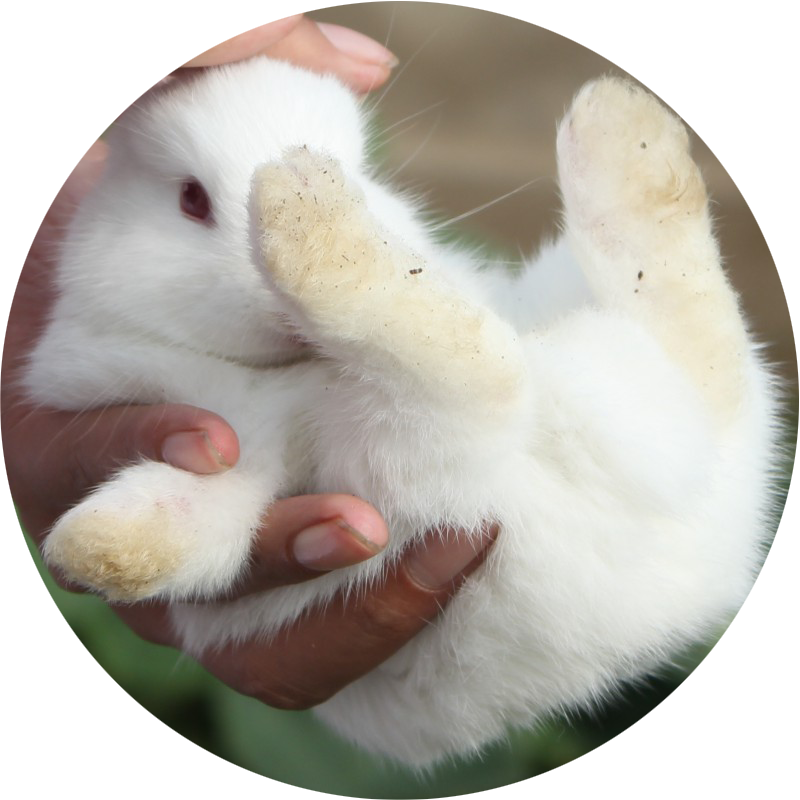
\includegraphics[width=2.8em]{headshot.png}\hspace{5.1em}
    \end{figure}

    \vspace{-1.5em}

    \hfill {\subsectionfont by\myauthor}\hspace{5em}

    \hfill {\subsectionfont \number\year.\number\month.\number\day} \hspace{4.8em}

    \vspace{2cm}
}

% 特殊符号和字体
\newcommand{\splitdot}{\dotfont ·}

\newcommand{\spell}[1]{{\spellfont #1}}

\newcommand{\tempsymbol}{{\tempfont℃}}

\newcommand{\chsline}{\hspace{0.15em}\rule[0.35em]{1.7em}{0.03em}\hspace{0.15em}}

% 章前注的参数
\newlength{\chapterblank}
\setlength{\chapterblank}{3cm}
\newcommand{\prenoteblank}{\vspace{1\baselineskip}}

% 章前注
\newcommand{\prenotes}[1]{
    {\prenotefont #1}\prenoteblank
}
\newcommand{\prenoteswith}[2]{
    {\prenotefont #1}

        {\rmfamily}#2\prenoteblank
}

% 扉页
\newcommand{\mytitlepage}{
    \
    \vfill
    \thispagestyle{empty}

    \begin{center}
        \Huge

        \titlefont

        {\mytitleen}

        \vspace{2mm}

        {\mytitle}

        \Large

        \vspace{60mm}

        {\cpfont\mycp}

        \vspace{2mm}

        {\signfont BY \myauthor}
    \end{center}

    \vfill

    \clearpage
}

% 尾页
\newcommand{\myendpage}{
    \newpage
    \ifodd\thepage
        \blankpage
    \fi

    \newpage

    \thispagestyle{empty}

    \

    \vfill

    \begin{minipage}{50mm}

        模板制作:兔子草

    \end{minipage}
    \vspace{5mm}
}

% 插入图片
\usepackage{graphicx}
\usepackage{float}

\usepackage[bottom]{footmisc}

\let\origpart\part
\renewcommand*{\part}[2][]{%
    \ifx\\#1\\% optional argument not present?
    \origpart{#2}%
        \renewcommand*\parttitle{#2}%
    \else
    \origpart[#1]{#2}%
        \renewcommand*\parttitle{#1}%
    \fi
}